% 編集した箇所
% 5.1機能概要、5.2前提条件、5.3制約事項、6.1人の流れ、7.想定する利用者

% 編集する必要がある箇所
% 1.はじめに、2.解決できる経営課題、3.課題解決のための提案、4.課題解決のための方法、6.2データの流れ、9.システムのハードウェア構成、15.1費用、15.2効果、16.アピールポイント、17.用語定義

% データの流れ:らず端末のときにログインできないけど、どうやってユーザ登録とかログインするの?
\documentclass[a4j,titlepage]{ujarticle}
\usepackage[dvipdfmx]{graphicx}
\usepackage{enumerate}
\usepackage{url}
\usepackage{listings}


\title{
{ローカル授業支援システム
\\
システム提案書}
\author{\\
\\
\\
\\
\\
Outing Corporation}
\date{\today}
}

\begin{document}
\maketitle


\tableofcontents

\clearpage

\section{はじめに}
% 課題提出型講義が今増えている
% 高知工科大学でもこういった講義がある
% その講義(実験)の概要
% 今の問題点
% その現状に対してのシステムの提案

大学では、講義内容の理解度の確認や講義外での予習・復習を促すため、講義当日の提出を求める課題を提示する課題提出型の講義が開講されることが多々あります。
課題提出型の講義の一例として、高知工科大学様で開講される情報学群実験第1、情報学群実験第2が挙げられます。これらの講義では、学生は個人、または小数人で構成されたグループに分かれ、講義内で提示された課題に取り組みます。その後、課題達成の確認を高知工科大学様が雇用したTeaching Assistant(以下TA)に依頼し、TAにより正式に課題の達成が認められます。
現在、学生が課題の確認をTAに依頼する際、学生は挙手によって確認依頼の意を表明し、TAを自席に呼び、学生自身の課題の進捗の報告と課題の確認依頼を口頭で説明する必要があります。また、課題に対する質問をする場合も、課題の確認と同様の手順でTAに依頼をしなければなりません。

課題達成の確認と質問のどちらの場合も挙手制であることは、TA及び学生にとって非効率であると考えられます。
TAは学生の口頭説明により、初めて課題の確認か質問か、そして質問であればどの課題に対してどのような疑問があるのか、ということを知ることができます。
講義終了直前であれば、課題の確認や質問のために挙手をする学生が増えるため、TAは講義内に達成を義務付けられた通常課題を終えた学生に与えられる発展課題の確認や質問を求める学生への対応よりも、通常課題の確認や質問を求める学生への対応を優先したいという考えがあるため、学生の課題の進捗状況を事前に確認できないことが問題となります。挙手をする学生の人数によっては、TAは学生の課題の進捗状況を聞いてから対応を後に回す必要もあります。
加えて、どこで学生が挙手をしているのかを把握しがたいという問題があります。
また、TAはどのような質問がされるのかわからないため、質問によっては学生に話を聞いてから回答や対応を考える必要があると考えられます。課題の問題文に対する質問があれば、TAは教授に課題の仕様を確認する場合もあります。これら質問は同講義で既出の質問であり、同じ質問が複数の学生から上がることもあります。
以上の問題を含め、学生の課題の提出が講義時間内で終わらないことが多々あります。

このような現状に対して、課題達成の確認や質問を効率よく行うことができる、課題提出型講義支援システムをご提案いたします。

\section{解決できる経営課題}
現在、高知工科大学様で開講される課題提出型の講義では、学生の課題達成が講義時間内に終わらない状況にあります。

その背景として、以下のような課題が挙げられます。
\begin{enumerate}[(1)]
\item 課題の確認と質問が挙手制であり、挙手をしている学生の視認および把握が困難
\item 学生の挙手が同一の時間に集中した場合、どちらを優先すべきかわからない
\item 挙手に抵抗のある学生がいるため、挙手が同一の時間に集中する要因となっている
\item 質問に関しても同様に挙手制であり、課題の確認との区別ができない
\item TAは学生の課題の進捗状況が分からないため、講義終了前に学生の支援を行うことが困難
\end{enumerate}
講義時間内に学生の課題の提出が終わらないことにより、TAの講義時間外の就労が数時間に及ぶことがあります。TAには時給が発生しているため、受講している学生全員の課題提出が終わらない限り、高知工科大学様がTAにお支払いする金額も大きくなると考えられます。

\section{課題解決のための提案}
本提案書では前項で述べた課題を解決するものとして「ローカル授業支援システム」を提案いたします。

\begin{enumerate}[(1)]
\item 学生からの課題の確認および質問のリクエストをまとめて可視化し、TAがスムーズに対応できる状況を提供します。
\item 学生からの質問は保存し、今後の講義に役立てることができます。
\item 各学生やグループの進捗状況を一覧で表示することで、TAが優先順位を考えて行動することができる状況を提供します。
\end{enumerate}

\section{課題解決のための方法}
前項で説明した提案につきまして、具体的な方法を説明いたします。
\begin{enumerate}[(1)]
\item 学生からの課題の確認および質問のリクエストをまとめ、課題の確認か質問のどちらをどの学生が行ったかを表示させる。
\item 学生からの質問は、データベースに蓄積させる。質問に対する回答を入力した場合は、質問は回答とともにデータベースに蓄積させることができる。TAは任意の折にデータベース上の質問と回答一覧を閲覧することができる。
\item 各学生やグループは課題の確認のリクエストとは別に、課題の進捗状況を選択し、送信する。
\end{enumerate}

\section{機能概要,前提条件,制約事項}

\subsection{機能概要}
\begin{enumerate}[(1)]
\item 学生が進捗状況を入力及び送信することで、管理者が学生全体の課題の進捗を把握することができます。
\item 学生が管理者に、質問や課題の確認のリクエストを送ることができます。
\item 管理者は、進捗管理画面の作成および編集、保存ができます。
\item 管理者は、過去の学生が送信した質問やデータの一覧を閲覧・編集することができます。 
\end{enumerate}

\subsection{前提条件}
\begin{enumerate}[(1)]
\item このシステムの管理者はユーザ登録をすること。
\item このシステムを利用する学生は、端末としてRaspberry piまたはスマートフォンのどちらかを使用すること。
\end{enumerate}

\subsection{制約事項}
\begin{enumerate}[(1)]
\item 管理者は、進捗管理画面をあらかじめ作成すること。
\item 管理者は、作成した進捗管理画面のデータを、学生が使用する端末で閲覧できるように送信すること。
\end{enumerate}

\section{サービス利用までの流れ}
\subsection{人の流れ}
このシステムの利用者は、管理者と授業を受ける学生の二通りとなります。

管理者は、スマートフォンやパソコン等の端末から、システム管理者として管理者用のwebページにログインします。
管理者用のホームページからは、学生が使用する端末で表示される進捗管理画面の作成ページ、授業時にリアルタイムで学生から送信されたデータを閲覧できるページ、データベースに蓄積された、過去の学生が送信したデータを閲覧できるページ、データベースの編集ページに遷移することができます。

進捗管理画面の作成を行うページでは、チェックボックスやボタン、フォーム等の用意されたパーツを組み合わせ、配置し、文章の入力を行うことで進捗管理画面の作成を行えます。ここでは、あらかじめシステムに用意された進捗管理画面のレイアウトの雛形を利用することができます。このレイアウトの雛形に進捗や質問、アンケート等の文章を入力することで簡単に画面の作成が行えます。作成した画面のレイアウト及び文章は保存されるため、編集することができます。

作成した進捗管理画面は、授業時に学生の端末に表示させて利用します。学生はスマートフォンまたはRaspberry pi端末からシステムにログイン後、表示された画面の指示に従って、授業時に提示された課題やそれに対する質問、回答を端末に入力し、送信します。学生がデータを送信するたびに、データ閲覧ページは更新されるため、管理者はリアルタイムで学生の入力状況を把握することができます。

また、管理者は、授業時に学生から送信されたデータをいつでも閲覧することができます。


%学生側は、各グループの代表一人が、そのシステムにログインします。
%そして、課題を行う中で進捗状況や質問を入力していきます。
%管理者側は、入力された情報を確認し、実験を円滑に進めます。

システムの運用・保守については管理者が行い、質問等のデータベースの編集も行うことができます。
障害が発生した場合は、システムの再起動を行うことで前回更新した状況まで戻すことで対応します。 % 例えばどんな障害?システム自体の再起動かアプリだけの再起動か?
\begin{figure}[h]

\centering
   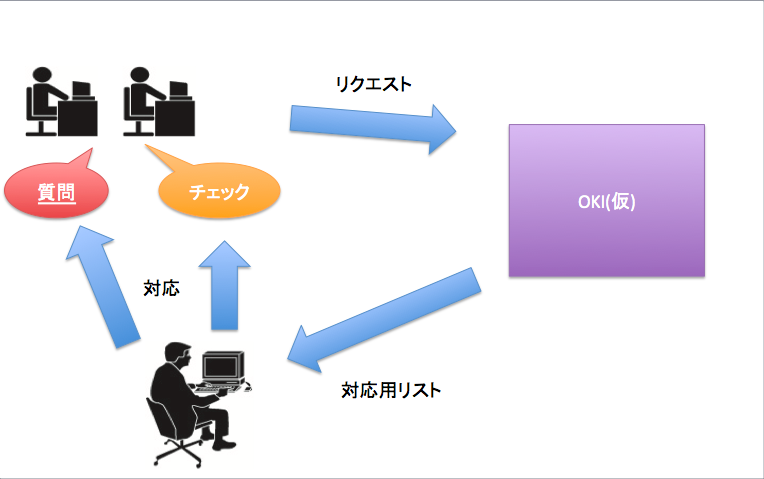
\includegraphics[width=13cm]{hito.png}
  \caption{主な流れ}
\end{figure}


\subsection{データの流れ}
このシステムは、ログイン画面によって管理者側と学生側の区別が行われます。そのため、システム自体は同様のものとなり、それとは別にサーバが % 学生側を利用者という言い方は良くない。ログイン画面で区別とは?システム自体が同様を別の言い方で
存在することでこのシステムの構成要素となります。
%システム内部での情報の流れは以下の図2のようになっています。 % どんな図作る?

サーバには学生側が登録の際に入力した個人情報や、質問の情報、課題の進捗状況などが格納されています。管理者は終了した講義の情報や次回の講義の
課題の情報を管理でき、利用者が前提条件に当てはまらなくなった場合には、登録の削除を行うことができます。
\begin{figure}[h]

\centering
   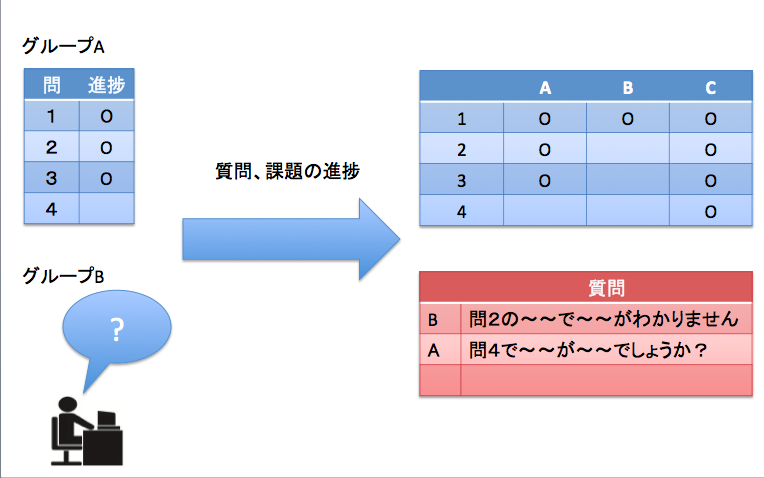
\includegraphics[width=13cm]{ui.png}
  \caption{データの集約の流れ}
\end{figure}

また、質問の一覧のデータを確認、削除することができ、そのデータベースの管理は管理者画面から行うことができます。

\section{想定する利用者}
このシステムが想定する利用者は、教育機関に就業する指導者やTA等の指導補佐、学生となっています。 % もうちょっと詳しく。どんな学生かとか。利用者を別の言い方にしたい。

\section{導入・移行計画}
2018年2月1日をもってアプリケーションの公開を完了します。

\section{システムのハードウェア構成}
システムのハードウェア構成は、メインサーバとしての役割をはたす Raspberry Pi 3 が1台、そのシステムを操作するコンピュータ端末が1台となっています。 % システムを管理する端末って何?ソフトウェア構成が書かれてないが、ソフトウェア構成とは何?

\section{運用・保守}
提案システムの運用・保守については、全て管理者が行います。 % 管理者って誰?<ーTAや教授 これまでに上手いこと説明できてたっけ?

\section{作業標準}
システム開発にかかる作業標準は貴校ご指定のものを使用します。

\section{品質管理}
システム開発にかかる品質管理は貴校ご指定のものを使用します。

\section{工程計画}
工程計画は次の通りです。

外部設計完了:2017年11月27日

内部設計完了:2017年12月18日

開発完了:2018年1月25日

導入:2018年2月5日

\section{体制}
このシステムの開発は弊社システム部門の沖を中心として、7名のエンジニアにより実施します。

\section{システム化にかかる費用とその効果}
\subsection{費用}
システム化にかかる費用は以下の通りです。

% 表どうしよう。誰か計算して~
\begin{table}[htb]
  \begin{tabular}{|c|c|c|c|c|} \hline
    項目 & 単価(円) & 数量 & 金額(円) & 備考 \\ \hline
     Raspberry Pi 3 &  5000&  1&  5000& x \\ \hline
     システム開発人件費&  2000& 90日x7人x3時間&3780000&x  \\ \hline
     周辺機器&  10000&  1&  10000&  \\ \hline
    \multicolumn{3}{|c|}{合計}& 3795000円 &  \\ \hline
  \end{tabular}
\end{table}

Raspberry Pi 3 に関しては、システムの運用に必要な台数は1台とし、その後必要に応じて追加で購入いただく
という形になっています。(この文いる?????)

%実験3c4cで平均残業時間が2時間で8人TAがいると考えると、合計672000の残業代がかかる。
%Raspberry Pi 3 が1台、周辺機器が1セット必要とすると、1万かかる
%そうすると、¥662000浮くはず で、開発人件費をどうするか
\subsection{効果}
今回例として挙げている高知工科大学情報学群実験では、1講義にTAが8人います。(言い方わからん)
現在TAの時給は1500円です。1クォーターに同じ講義は14回程度あります。以上のことをふまえた上で、
1講義あたりの平均短縮時間ごとの削減コストが図3となります。
\begin{figure}[h]

\centering
   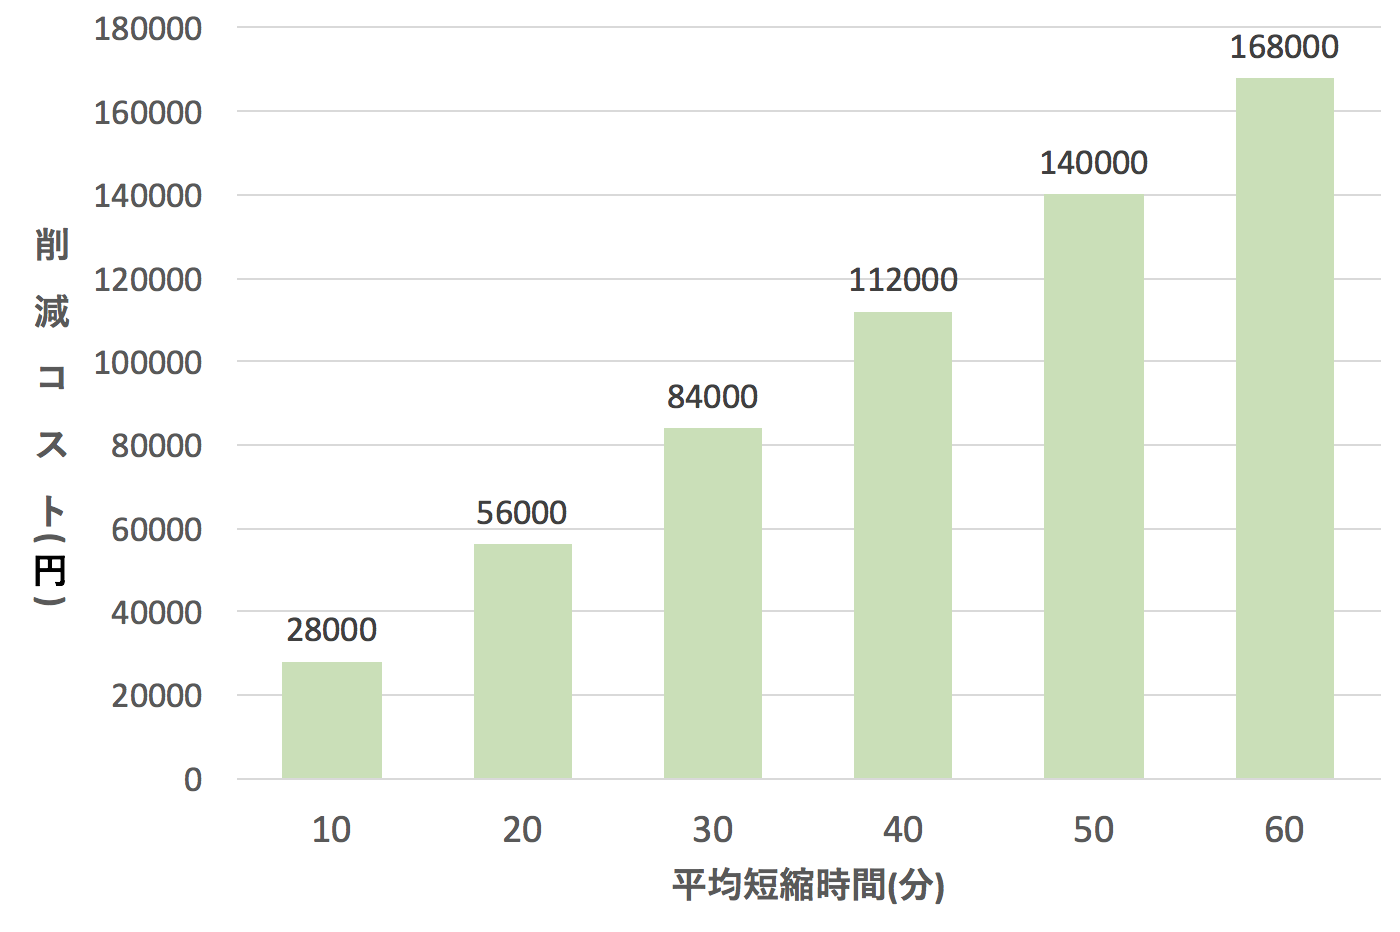
\includegraphics[width=13cm]{sisan.png}
  \caption{平均短縮時間とそれによる削減コスト}
\end{figure}

1講義あたり、30分短縮できると、TAのコスト(残業代としていいのか)が84000円削減されます。

%効果の試算として、TAの授業後の平均残業時間が2時間とし、TAがその講義に8人ついていたとします。
%現在のTAの時給は1,500円なので、1講義あたり8人 × 1,500円 × 2時間 で、1講義あたり24000円となります。
%そして、1クォーターに同じ講義は14回程度あるので、 24,000円 × 14回となり、一つの講義で336,000円のコストが削減されます。

このシステムを活用する講義の例として情報学群実験を挙げていますが、
情報学群実験は年間6講義あるので、 84000円 × 6講義 = 504000円が年間で削減されます。
このシステムを5年間運用すると、504000 × 5年 = 252000円のコストの削減が見込まれます。
また、学生が課題にかける時間も短くなるため、学習コストの削減にもつながり(学習コストは削減という形であっているのか)、
〜〜と学生の二者にとって利益をもたらすものだと考えられます。

\section{本システム提案のアピールポイント}
%汎用性の高いシステムとなっているため、他の会議等での利用も可能です。
質問の内容が蓄積され、次年度の講義の改善へ繋げることができます。
Raspberry-pi 3 をサーバとして使用しているので、あらゆる場所で使用することができます。
場所を取らず比較的容易に導入できることで、導入、運用共に安価です。(文章要考察)


\section{用語の定義}
TA :「Teaching Assistant」の略称で、授業のアシストをする大学院生のこと。

管理者 : 教授やTAのこと。




\newpage

\end{document}
